\section{Electrical Breakdown in High Voltage Systems} %Possibly a better heading needed
There are some consequences that need to be taken into account when designing system in high voltage. High voltage systems have much higher electric potential to their surrounding objects which are usually at earth potential, these arise electric potential gradient or electric field between the systems and their surrounding objects. The values of electric field can be extremely high due to the high voltage and may cause electrical breakdown and partial discharge which can lead to failure in systems. It is important to design systems to minimise the chance of these events.
\begin{figure}[!h]
   \centering
   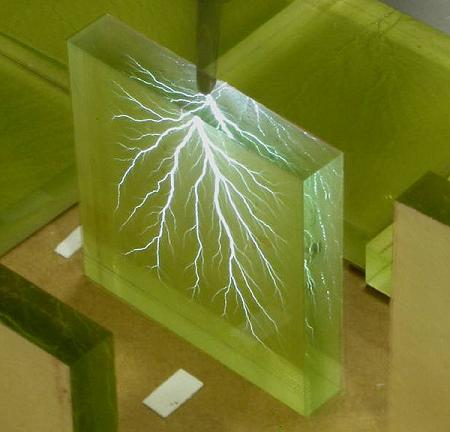
\includegraphics[width = 0.5\textwidth]{lichtenberg-figures004.jpg}
   \caption{Electrical tree tracing the path of damaged insulation caused by electrical breakdown}
   \label{figure:breakdown}
\end{figure}
%http://damnamazing.blogspot.co.uk/2008/11/captured-lightning-lichtenberg-figures.html
Electrical breakdown is the action of electrical conduction across a insulating medium, usually dielectric, when the voltage across this medium exceeds the breakdown voltage subject to the type of material of the insulation. This usually happens when the potential difference is extremely high and arcing can be seen in gaseous insulating medium. This can cause changes to the compounds in the insulating medium and also cause damage to equipments in systems as shown in figure \ref{figure:breakdown}. For example, breakdown in oil insulation due to excessive electric field.

There are different types of electrical breakdown. The main types of electrical breakdown that are involved in high voltage insulation systems are corona discharge in air and partial discharge in dielectric insulation.

\begin{figure}[!h]
   \centering
   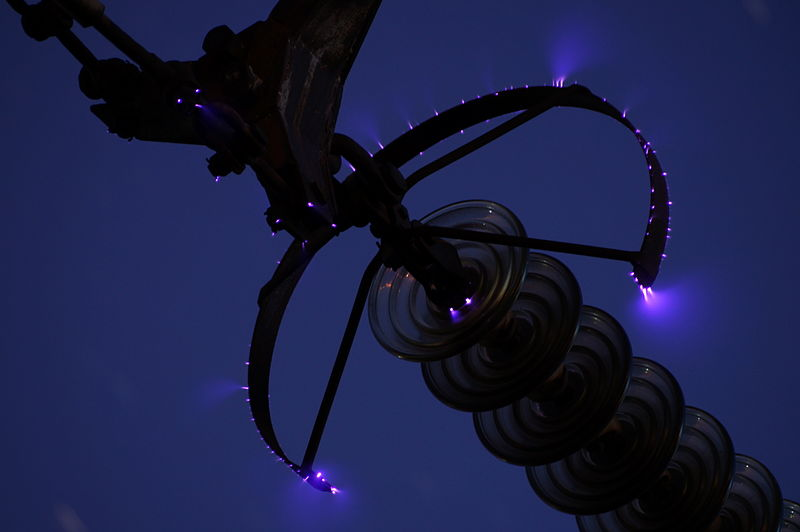
\includegraphics[width = 0.5\textwidth]{coronadischarge.jpg}
   \caption{Corona discharge appearing on the insulation surface of high voltage conductor}
   \label{figure:corona}
\end{figure}
%Problem, this picture is from wikipedia

\subsection{Corona Discharge}
Corona discharge is the ionisation of fluid around a conductor of high electric potential. The ionisation of the surrounding fluid is due to the discharge from the conductor. In high voltage systems, corona discharge occurs most commonly from the conductor to air surrounding the conductor as illustrated in figure \ref{figure:corona}. Corona discharge occurs at area of intense electric field, but not sufficiently intense to cause arcing. This type of breakdown might not cause fatal damage to the insulation, but would shorten the life time of the insulation system. Also, it is power loss to the surrounding, so it is important to design insulation system to minimise the effect of corona discharge.

\subsection{Partial Discharge}
Partial discharge is the electrical breakdown in small portion of dielectric material due to imperfection in the material. The most common cause of partial discharge is void with in the dielectric material, where these void contains material of a lower electrical breakdown strength then the dielectric material. Under high voltage applied across the dielectric insulation, these voids will experience local electrical breakdown if the corona inception voltage is exceeded, another words partial discharge in the dielectric insulation. Partial discharge can also occur under intense tangential electric field (electric field along the surface) and electron emission results \cite{surfaceflashover}, which is also known as surface flashover. In order to ensure the insulation system can sufficiently reduce the chance of surface flashover, the inception voltage of the insulation must be relatively high compare to the operating voltage of the conductor.